\appendix
\renewcommand{\cftchappresnum}{Appendix }
\apendixStyle
\apendixSecStyle



\chapter{PCB Schematics}
%\addcontentsline{toc}{chapter}{ WHIP Schematics }
% cropped pdfs with http://croppdf.com/
\label{chap:PCB_Schematics}
\begin{figure}
	\begin{center}
		\label{fig:FullSchematic_Sheet1}
			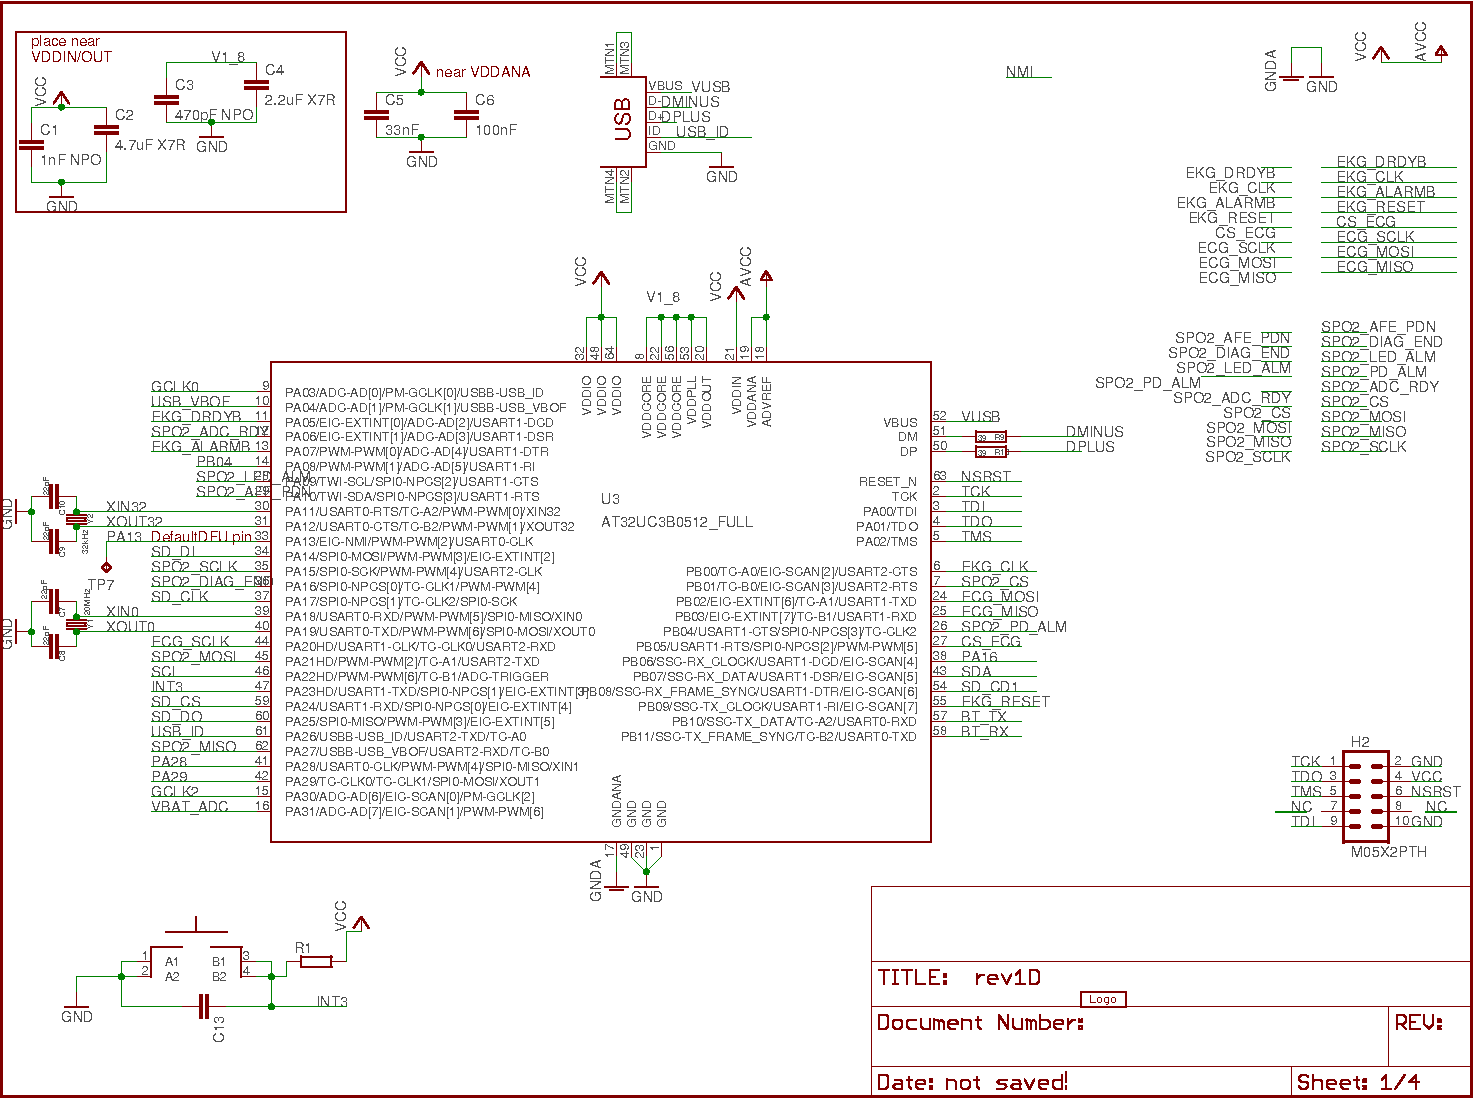
\includegraphics[angle=90,scale=1,width=1\textwidth]{Images/rev1D_sheet1-cropped.pdf} 
		\caption{Full Schematic, Microprocessor View}
	\end{center}
\end{figure}

\begin{figure}
	\begin{center}
		\label{fig:FullSchematic_Sheet2}
		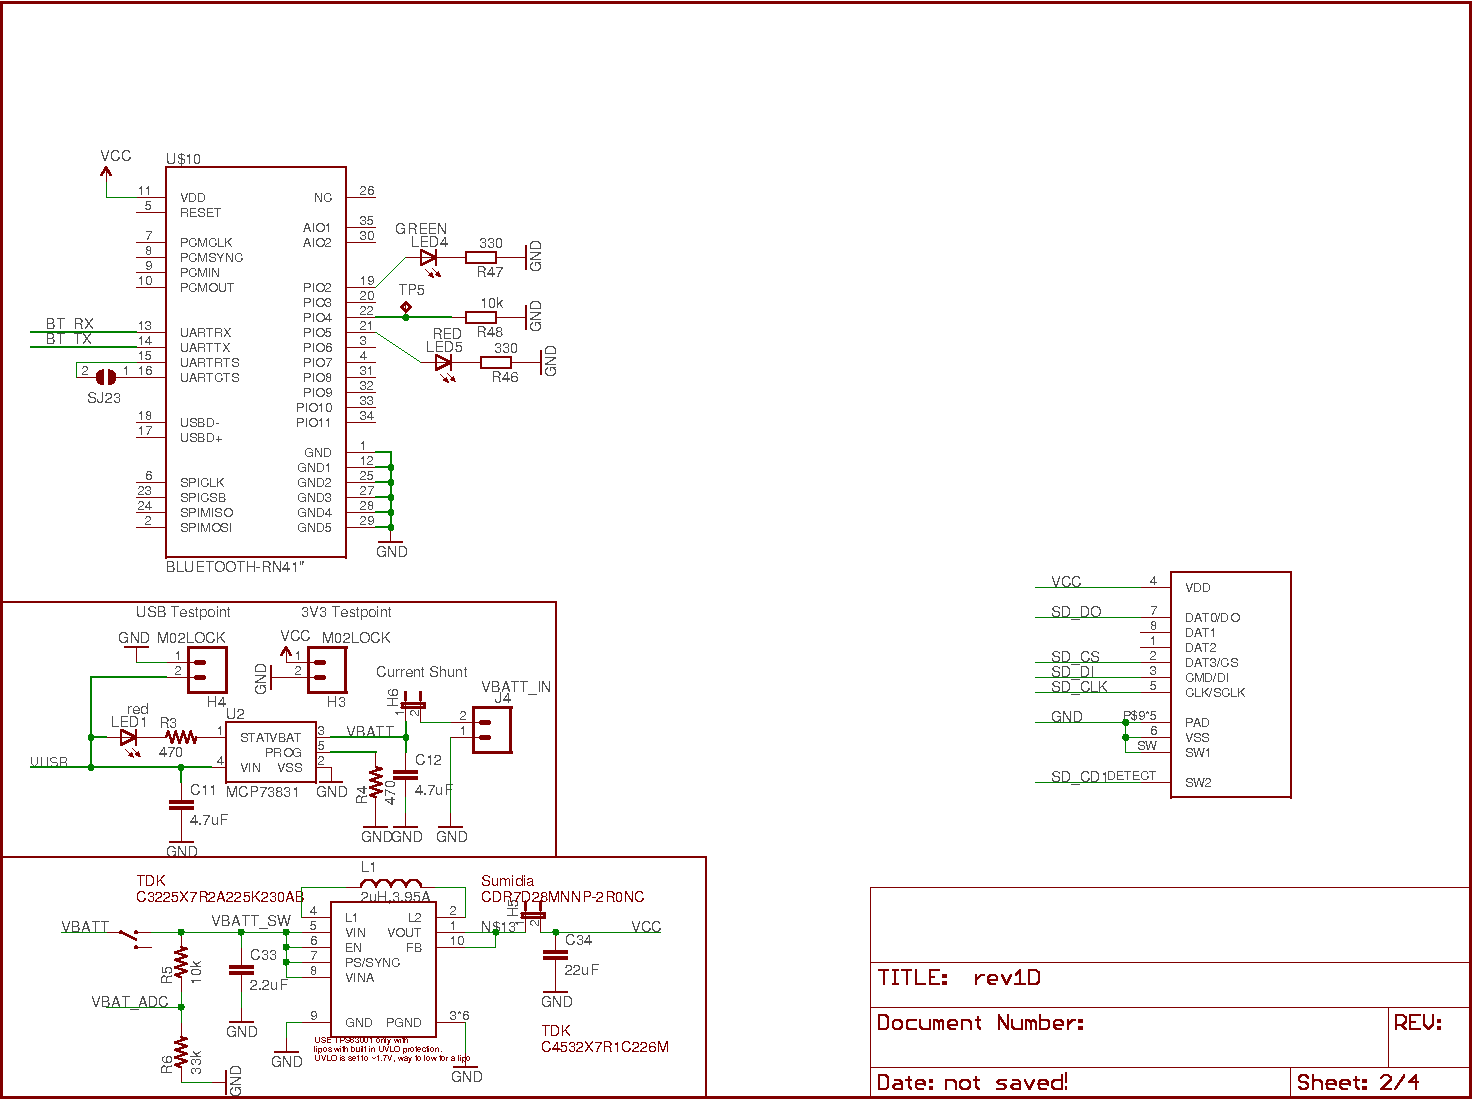
\includegraphics[angle=90,scale=1,width=1\textwidth]{Images/rev1D_sheet2-cropped.pdf} 
		\caption{Full Schematic, Bluetooth, Power System, and SD Card View}
	\end{center}
\end{figure}

\begin{figure}
	\begin{center}
		\label{fig:FullSchematic_Sheet3}
		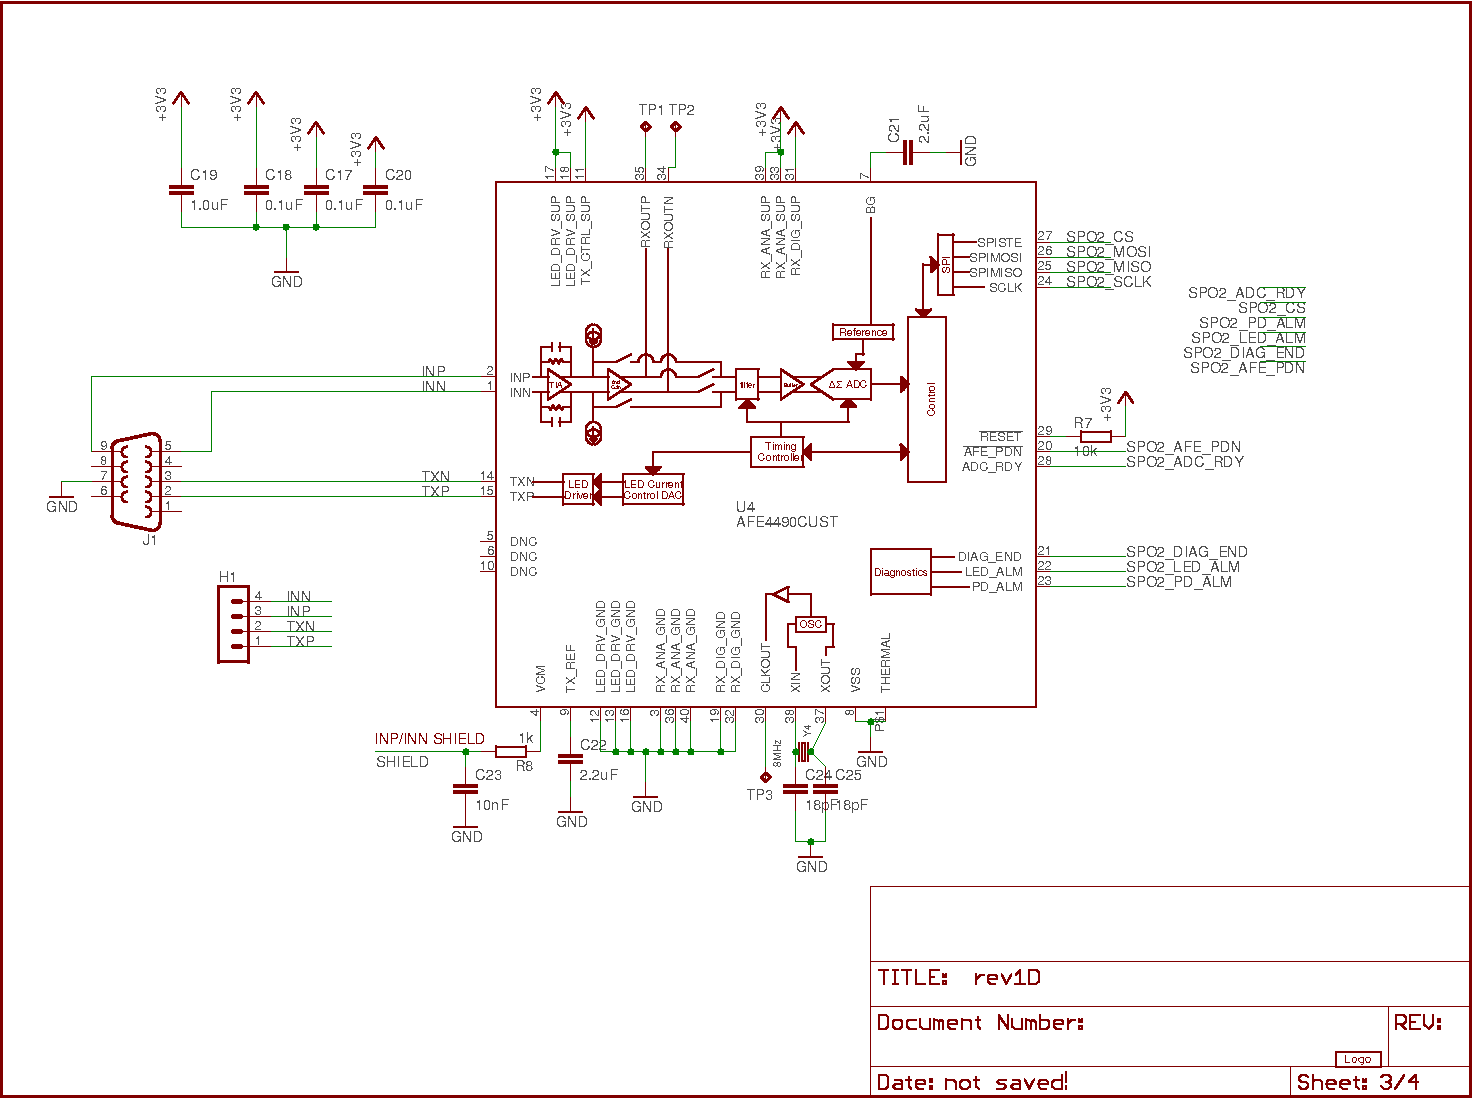
\includegraphics[angle=90,scale=1,width=1\textwidth]{Images/rev1D_sheet3-cropped.pdf} 
		\caption{Full Schematic, \spo2 View}
	\end{center}
\end{figure}

\begin{figure}
	\begin{center}
		\label{fig:FullSchematic_Sheet4}
		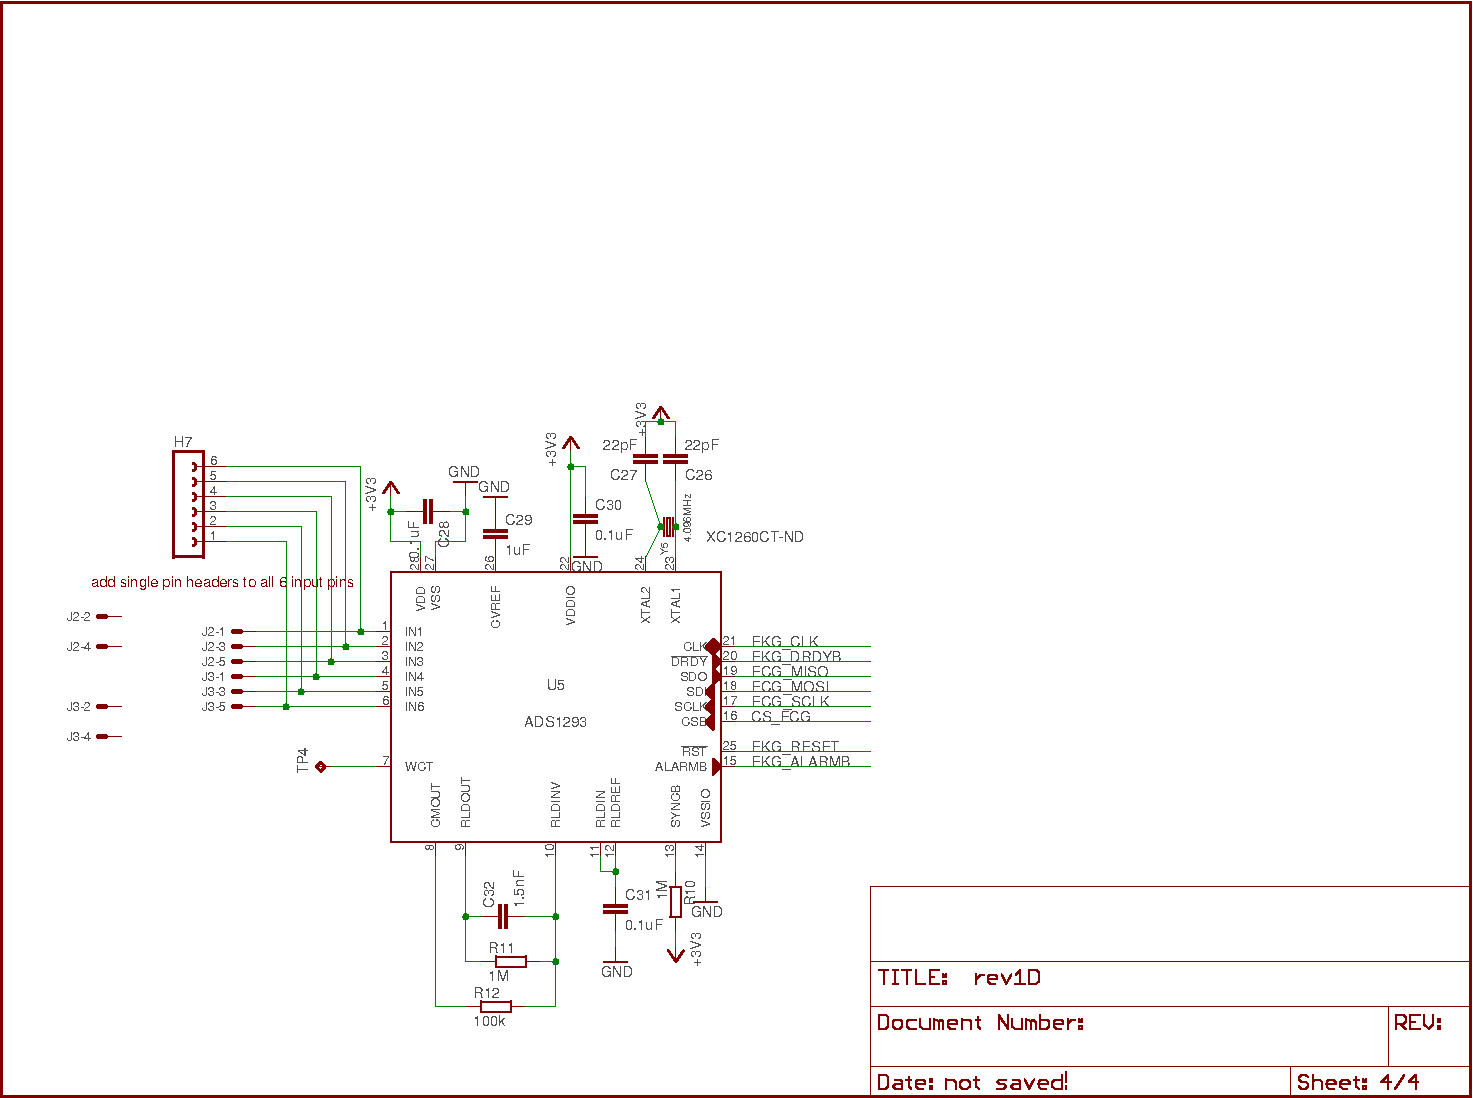
\includegraphics[angle=90,scale=1,width=1\textwidth]{Images/rev1D_sheet4-cropped.pdf} 
		\caption{Full Schematic ECG View}
	\end{center}
\end{figure}

\chapter{PCB Layout}


% %\addcontentsline{toc}{chapter}{ WHIP Layout }
\label{chap:PCB_LAYOUT}

\begin{figure}
\begin{center}
	\label{fig:TOPGerber}
	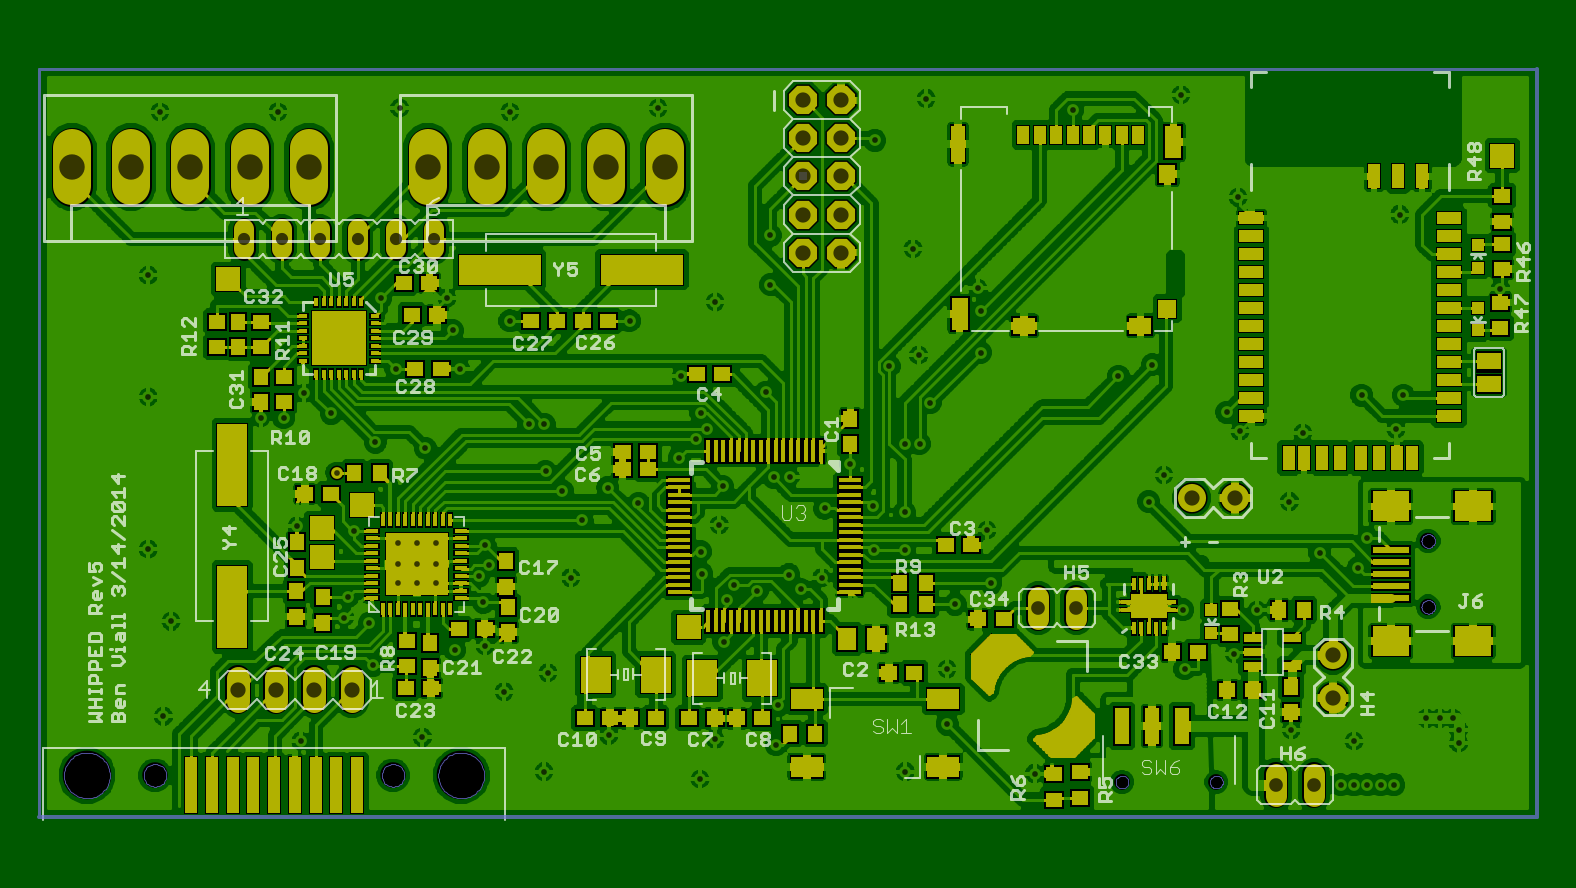
\includegraphics[angle=0,scale=1,width=.95\textwidth]{Images/Rev5_TOPGERB.png} 
	\caption{Gerber Render for Top Layer}
\end{center}
\end{figure}


\begin{figure}
\begin{center}
	\label{fig:BOTGerber}
	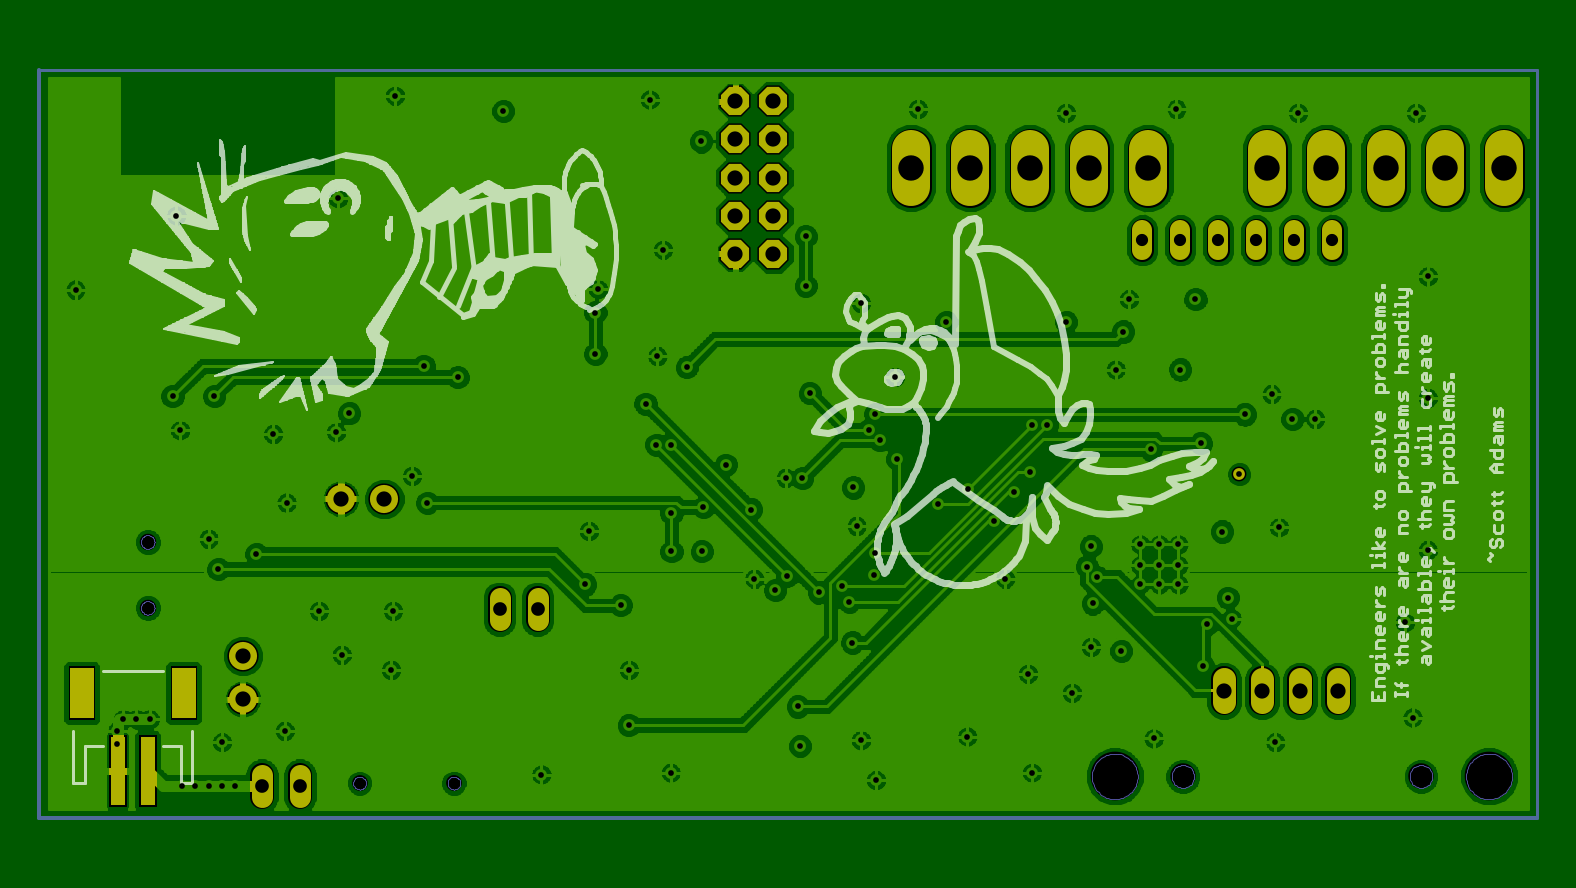
\includegraphics[angle=0,scale=1,width=.95\textwidth]{Images/Rev5_BOTGERB.png} 
	\caption{Gerber Render for Bottom Layer}
\end{center}
\end{figure}


\begin{figure}
\begin{center}
	\label{fig:GNDGerber}
	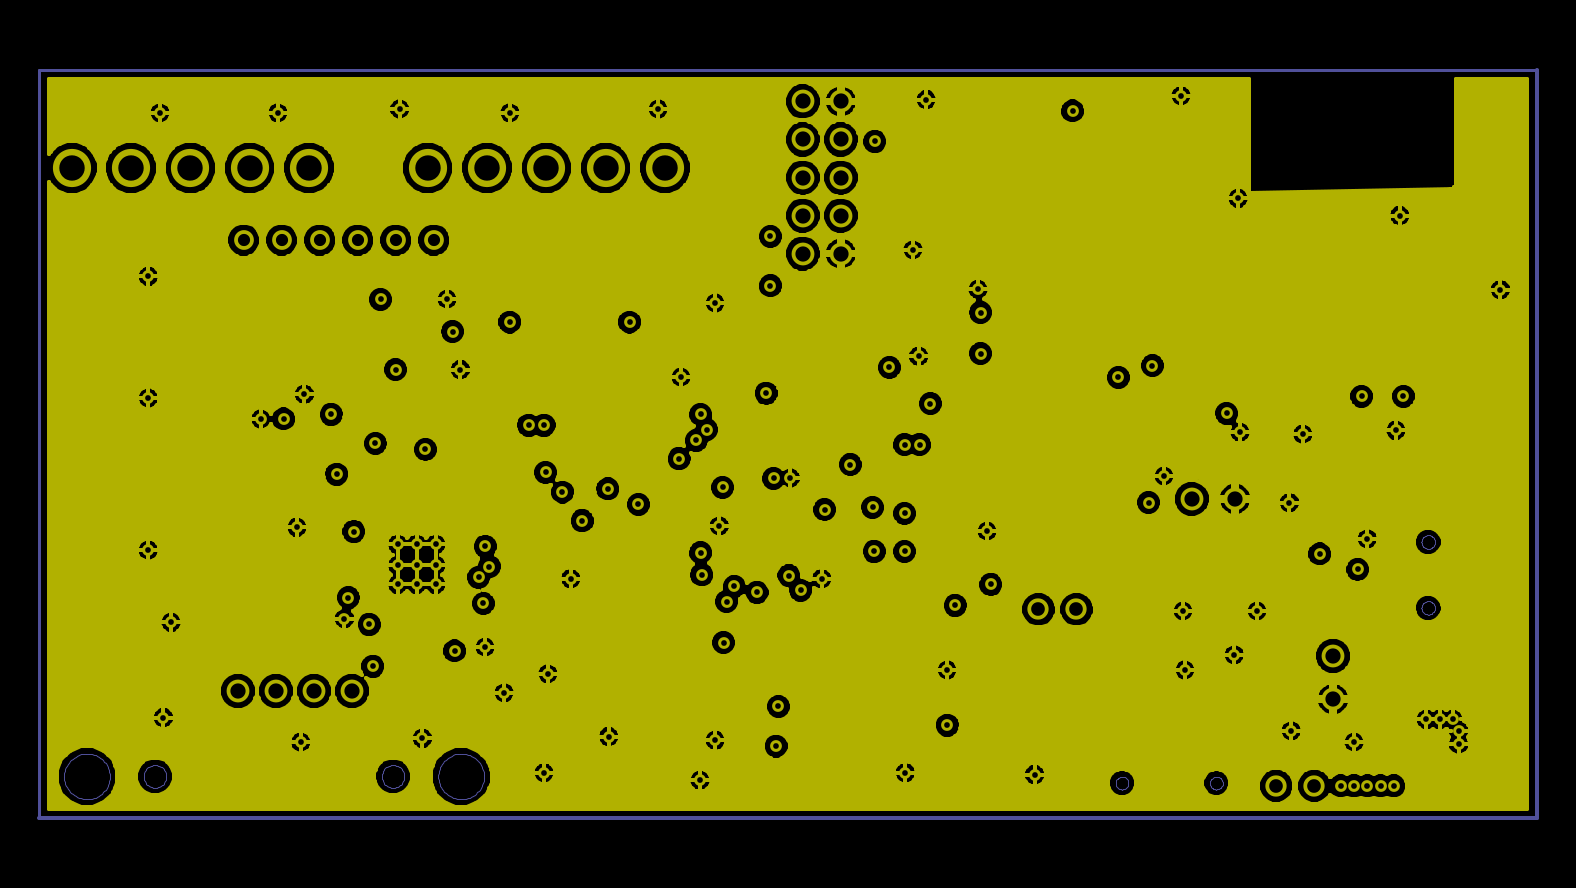
\includegraphics[angle=0,scale=1,width=.95\textwidth]{Images/Rev5_GNDGERB.png} 
	\caption{Gerber Render for Internal Ground Layer}
\end{center}
\end{figure}


\begin{figure}
\begin{center}
	\label{fig:PWRGerber}
	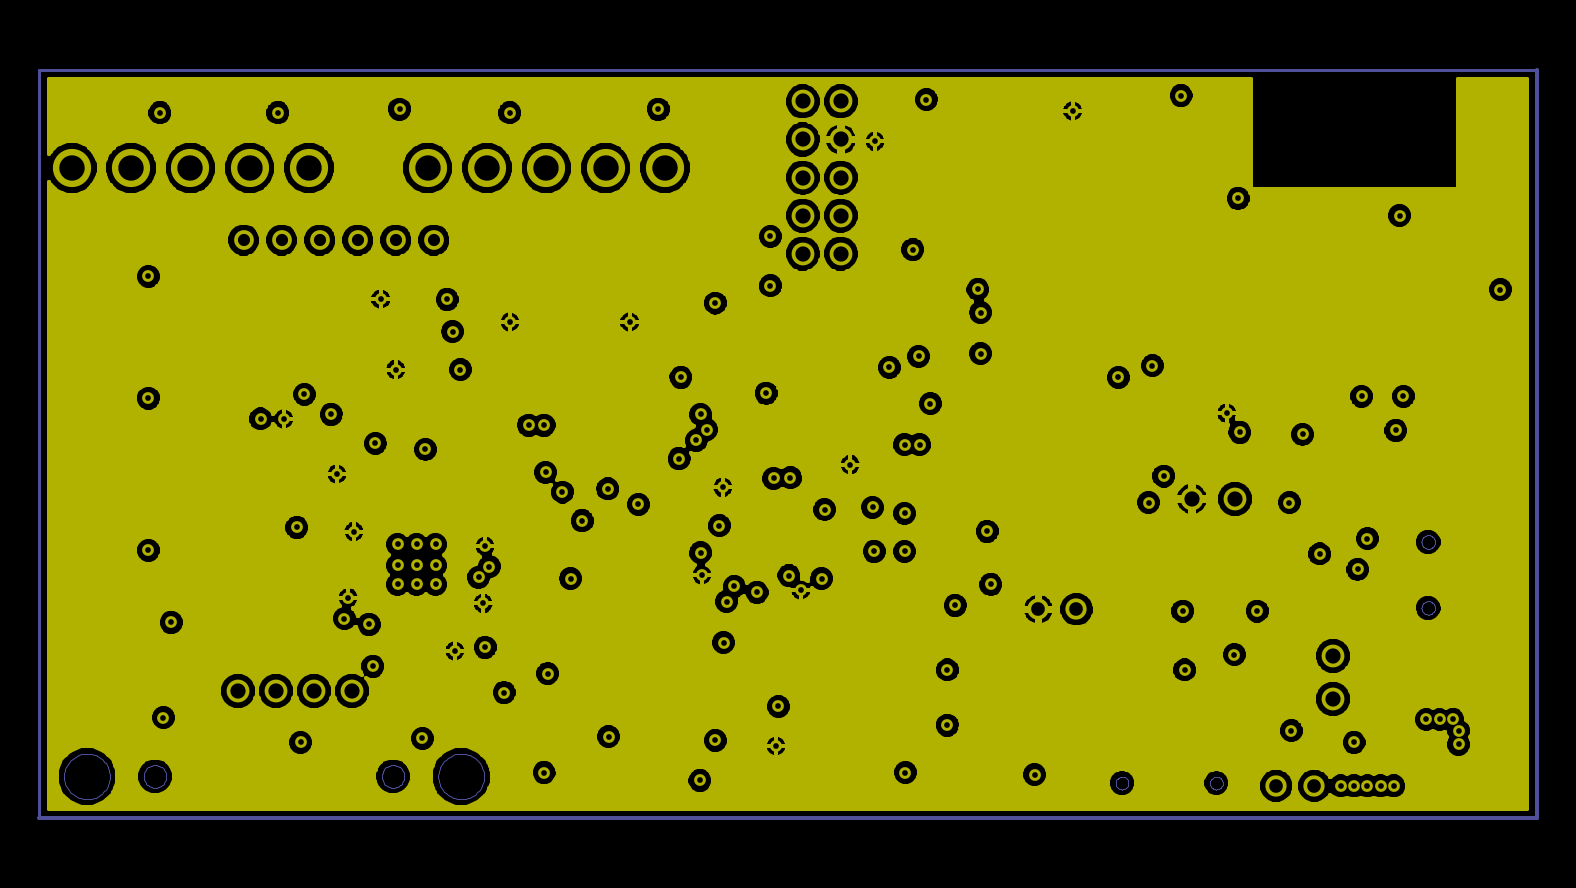
\includegraphics[angle=0,scale=1,width=.95\textwidth]{Images/Rev5_PWRGERB.png} 
	\caption{Gerber Render for Internal Power Layer}
\end{center}
\end{figure}


\newcommand{\putOversized}[7]{
\ifnum1=#6\relax
	\raggedright\noindent\bfseries\Large Appendix \ref{#1} (Cont.) \par
\fi
	\raggedright\fbox{\includegraphics[ #5,page=#3,width=#7]{#2}}
	
\ifnum1=#4\relax
	\normalfont\normalsize \parbox{#7}{\raggedleft(cont. on next page)} \par
\fi
\raggedright\clearpage
}

\chapter {Institutional Research Board (IRB) Material}
\section{Permission Letter}
\label{sec:permissionLetter}
\setlength{\fboxsep}{0pt}

%\fbox{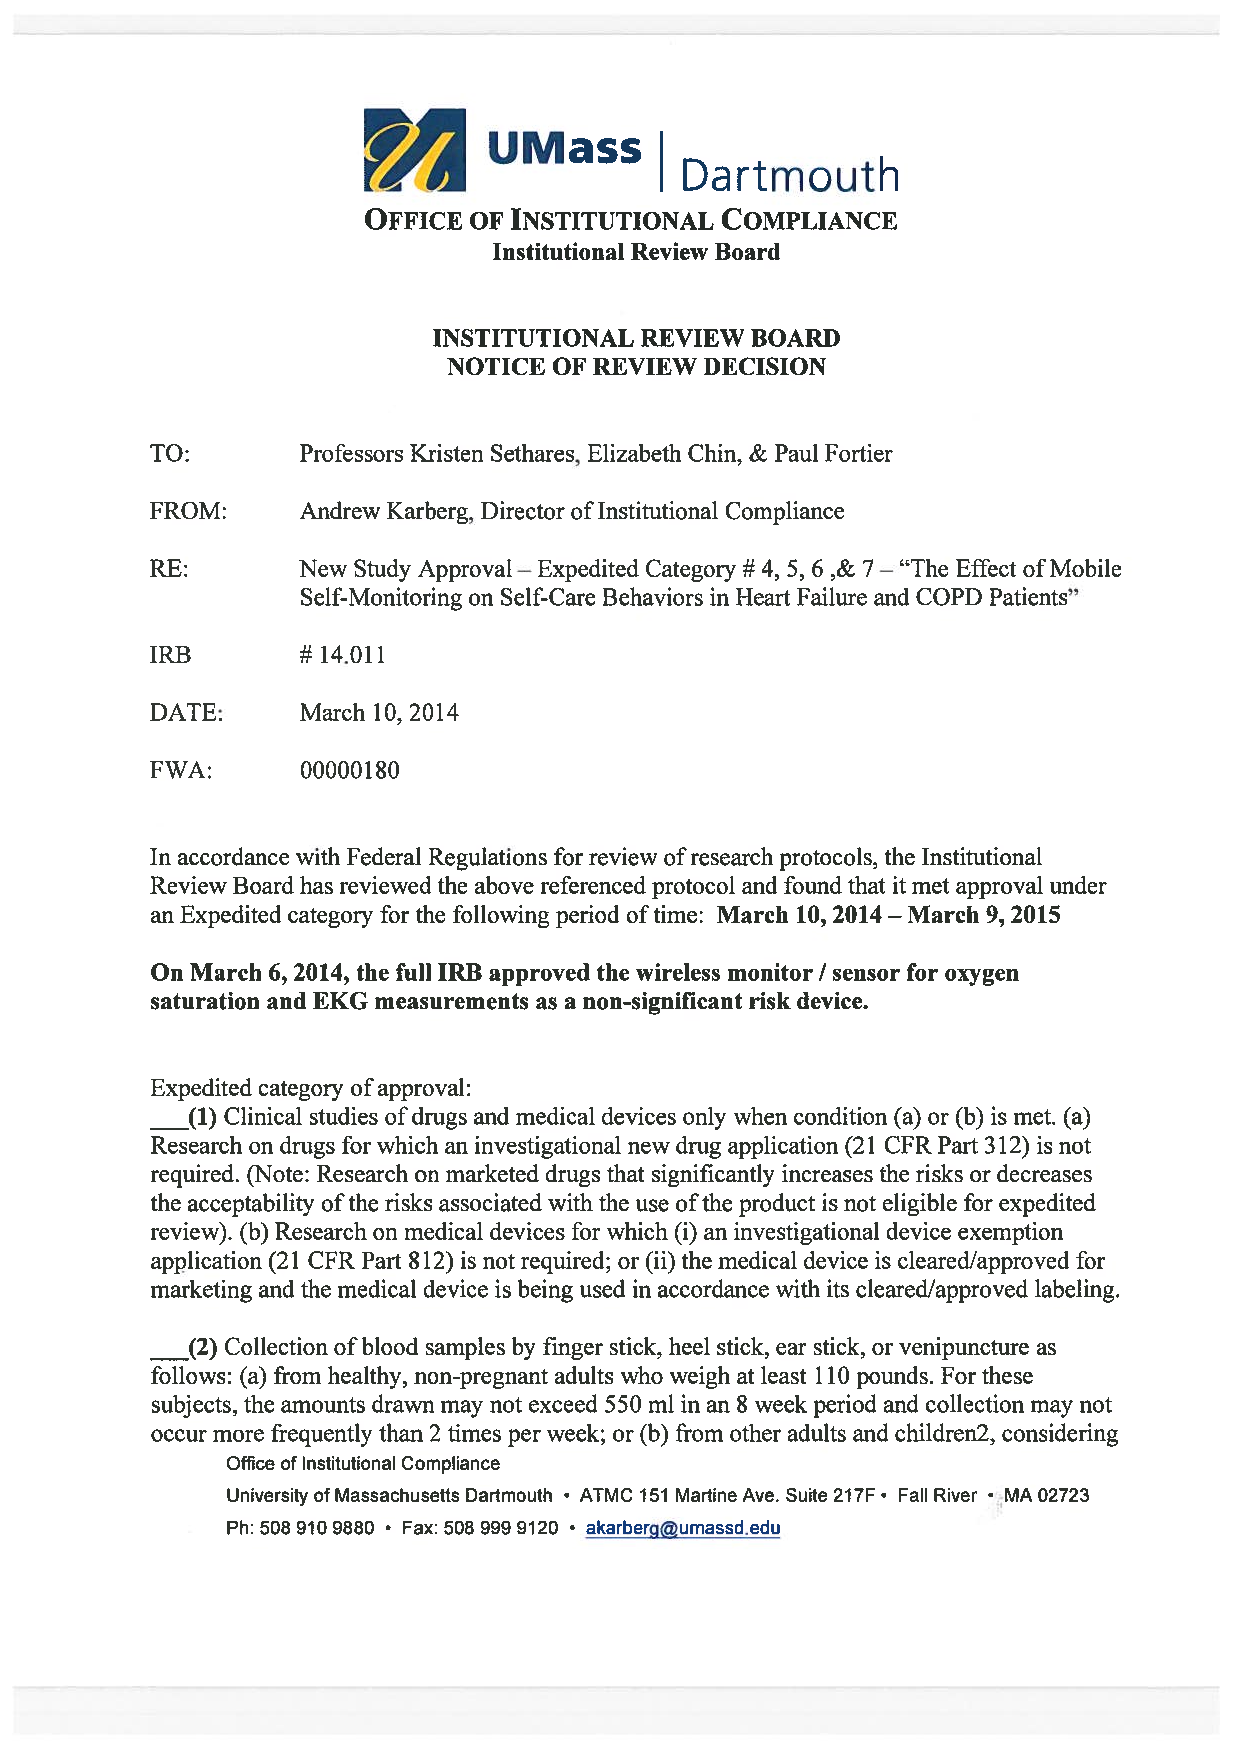
\includegraphics[trim= 0mm 20mm 0mm 16mm,clip,page=1,width=\textwidth]{Images/IRB_Form.pdf}}
%\OversizeContinued

														%       L   B    R   T   
\putOversized{sec:permissionLetter}{Images/IRB_Form.pdf}{1}{1}{trim = 0mm 25mm 0mm 16mm,clip}{0}{\textwidth}
\putOversized{sec:permissionLetter}{Images/IRB_Form.pdf}{2}{1}{trim = 0mm 20mm 0mm 16mm,clip}{1}{\textwidth}
\putOversized{sec:permissionLetter}{Images/IRB_Form.pdf}{3}{1}{trim = 0mm 20mm 0mm 16mm,clip}{1}{\textwidth}
\putOversized{sec:permissionLetter}{Images/IRB_Form.pdf}{4}{1}{trim = 0mm 20mm 0mm 16mm,clip}{1}{\textwidth}
\putOversized{sec:permissionLetter}{Images/IRB_Form.pdf}{5}{1}{trim = 0mm 20mm 0mm 16mm,clip}{1}{\textwidth}
\putOversized{sec:permissionLetter}{Images/IRB_Form.pdf}{6}{1}{trim = 8mm 35mm 8mm 20mm,clip}{1}{\textwidth}
\putOversized{sec:permissionLetter}{Images/IRB_Form.pdf}{7}{1}{trim = 8mm 35mm 8mm 20mm,clip}{1}{\textwidth}
\putOversized{sec:permissionLetter}{Images/IRB_Form.pdf}{8}{0}{trim = 8mm 35mm 8mm 20mm,clip}{1}{\textwidth}
%\putOversized{sec:permissionLetter}{Images/IRB_Form.pdf}{9}{0}{0mm 35mm 0mm 20mm}
%\fbox{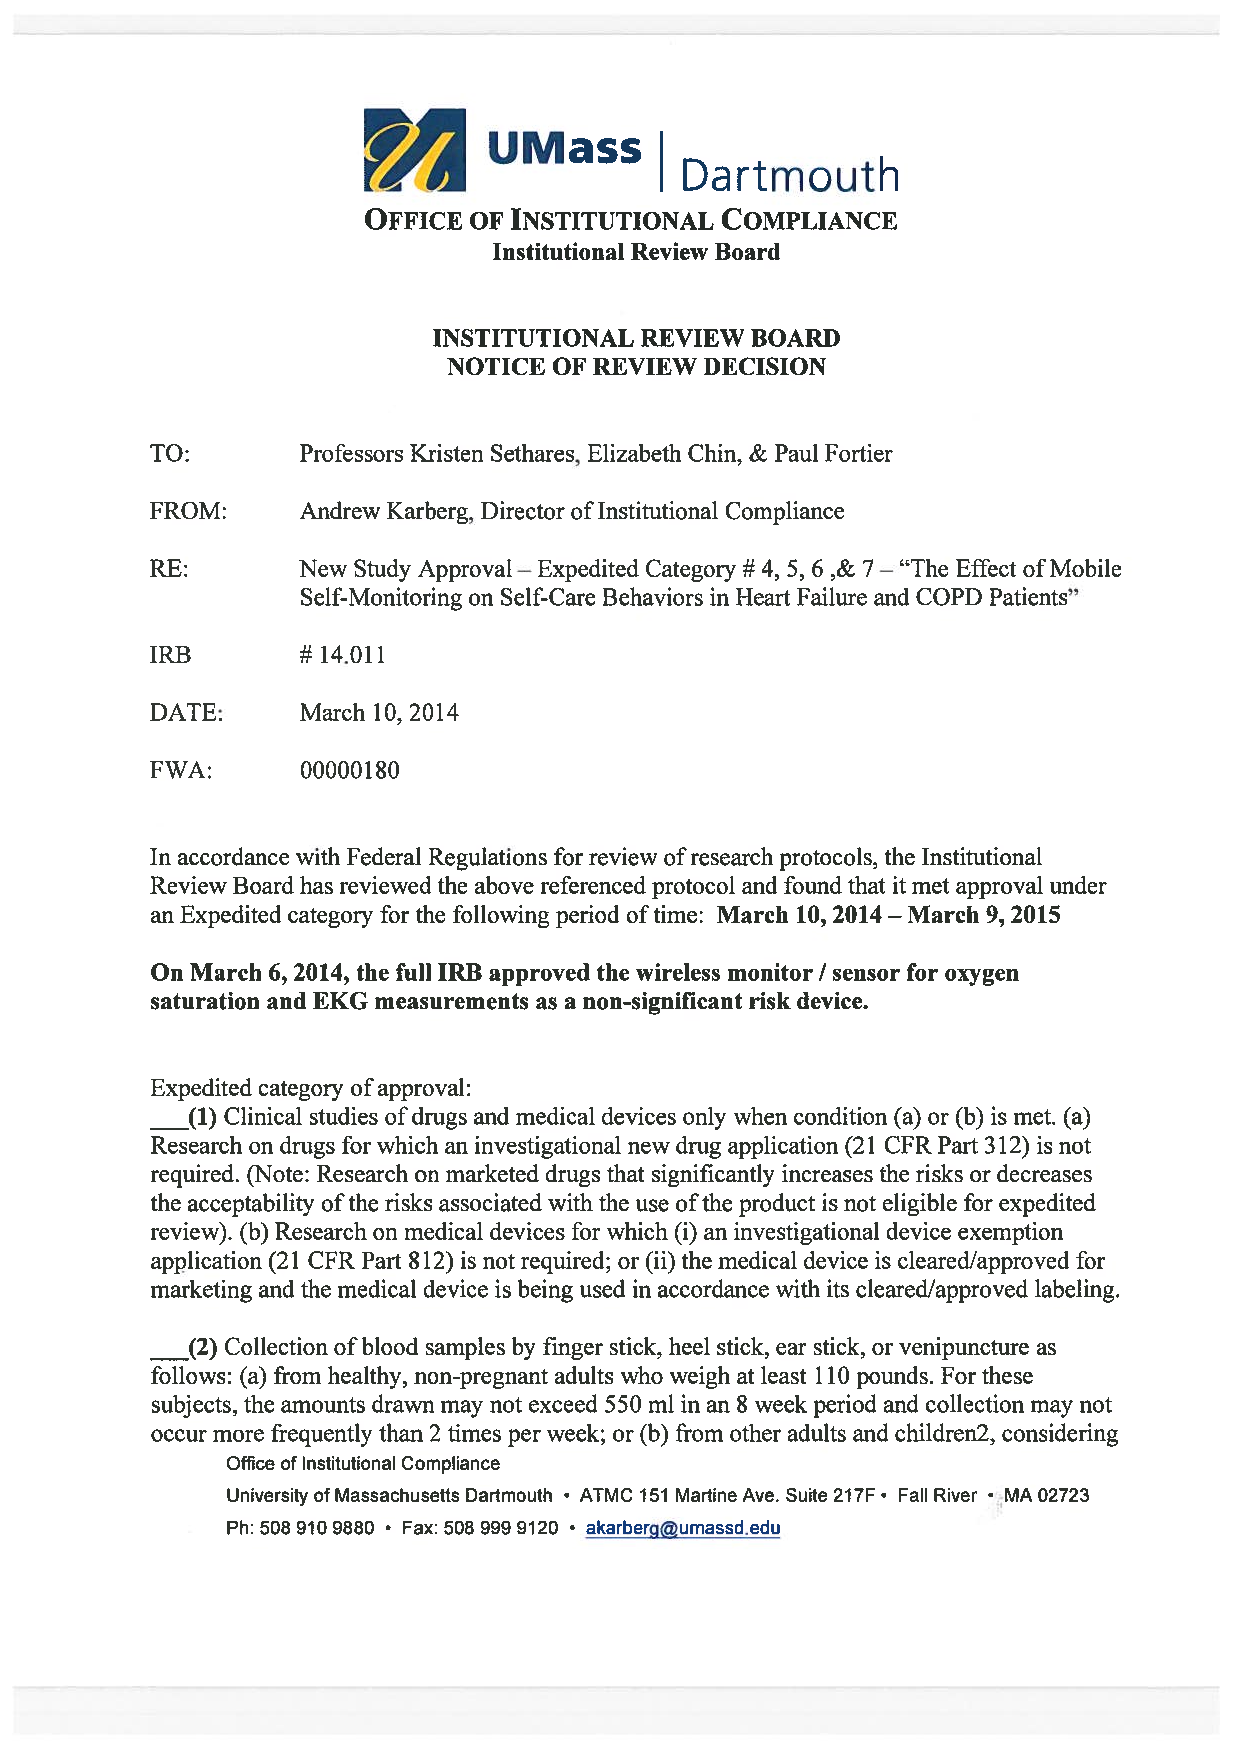
\includegraphics[trim= 0mm 20mm 0mm 16mm,clip,page=1,width=\textwidth]{Images/IRB_Form.pdf}}
%\OversizeContinued

%\bfseries\Large\Cref{sec:permissionLetter} (Cont.) \\\vspace{2pt}
%\fbox{\includegraphics[trim= 0mm 20mm 0mm 20mm,clip,page=2,width=\textwidth]{Images/IRB_Form.pdf}}
%
%\fbox{\includegraphics[trim= 0mm 20mm 0mm 20mm,clip,page=3,width=\textwidth]{Images/IRB_Form.pdf}}

%\fbox{\includegraphics[trim= 0mm 20mm 0mm 20mm,clip,page=4,width=\textwidth]{Images/IRB_Form.pdf}}

%\fbox{\includegraphics[trim= 0mm 20mm 0mm 20mm,clip,page=5,width=\textwidth]{Images/IRB_Form.pdf}}

%\includepdf[offset= .3in 0in,frame,trim= 0mm 35mm 0mm 20mm,clip, pages={6-},width=\textwidth]{Images/IRB_Form.pdf}


\section{Duke Activity Status Index} 
\fbox{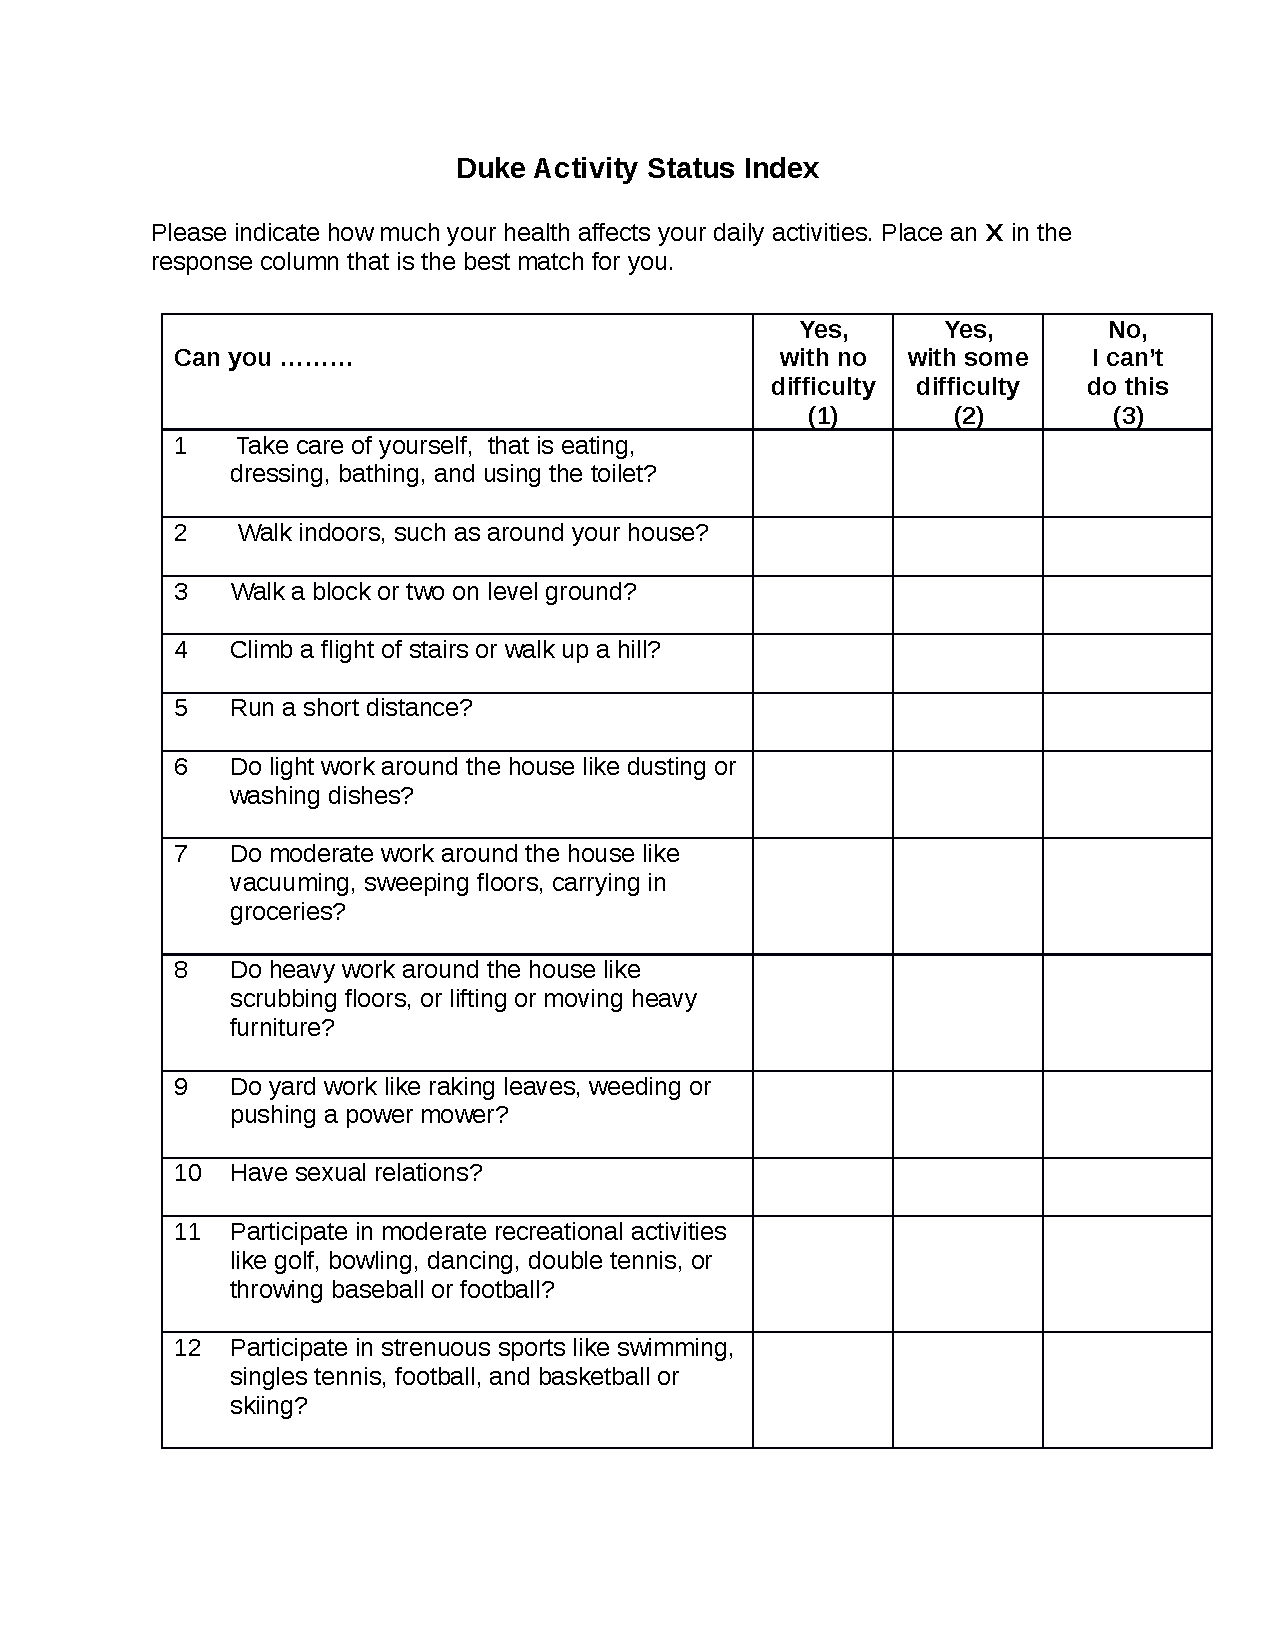
\includegraphics[page=1,width=.95\textwidth]{Images/DASI_form.pdf}}

\section{Heart Failure Somatic Awareness Scale}
\label{sec:HFSAscale}
\putOversized{sec:HFSAscale}{Images/HFSA_Form.pdf}{1}{1}{angle=90}{0}{.9\textwidth}
\putOversized{sec:HFSAscale}{Images/HFSA_Form.pdf}{2}{1}{angle=90}{1}{.9\textwidth}
\putOversized{sec:HFSAscale}{Images/HFSA_Form.pdf}{3}{0}{angle=90}{1}{.9\textwidth}
%\fbox{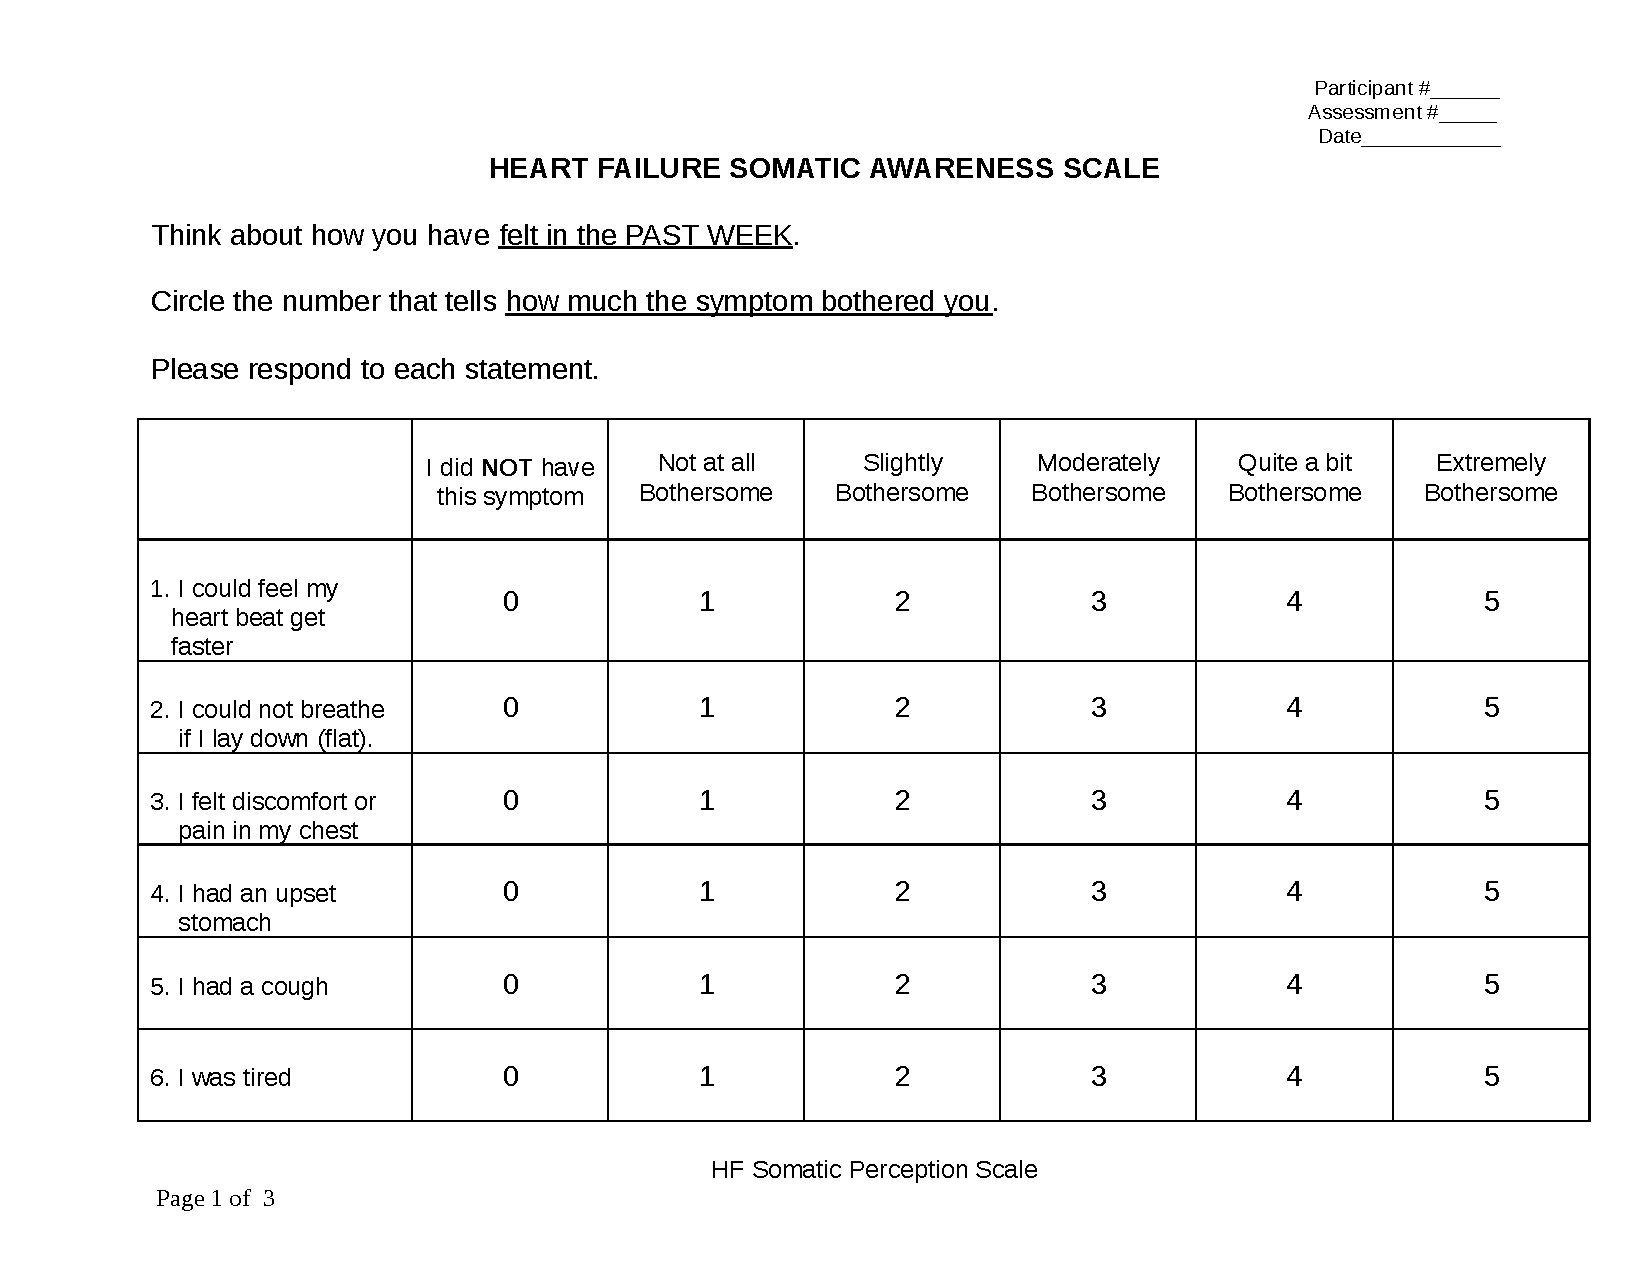
\includegraphics[page=1,angle=90,width=.95\textwidth]{Images/HFSA_Form.pdf}}
%\noindent Continued on Next Page

%\section*{Heart Failure Somatic Awareness Scale (cont.)}
%\noindent\fbox{\includegraphics[page=2,angle=90,width=.95\textwidth]{Images/HFSA_Form.pdf}}

%\noindent Continued on next Page

%\section*{Heart Failure Somatic Awareness Scale (cont.)}
%\noindent\fbox{\includegraphics[,page=3,angle=90,width=.95\textwidth]{Images/HFSA_Form.pdf}}

%\cftaddtitleline{toc}{chapter}{Source Code}{Back Pocket}
\chapter{Source Code: CD Back Pocket}
